\documentclass[compress]{beamer}  % compress diminui o tamanho da barra de navegacao
\mode<presentation>
\graphicspath{ {images/} }
%\usetheme{Madrid}
%\usetheme{Copenhagen}
\usetheme{Dresden}

\setbeamertemplate{mini frames}[default]


\usepackage[utf8]{inputenc}
\usepackage{ifthen}		% pacote usado no logo (mudar o logo apos o primeiro slide)
\newboolean{front}
\setboolean{front}{true}

 
 
%Information to be included in the title page:
\title{Mechanistic numerical modelling of solute uptake by plant roots}
\author[Bezerra, A.H.F.]
{
Andre Herman Freire Bezerra\\
{\scriptsize Advisor: Quirijn de Jong van Lier}
}

\institute{University of S\~ao Paulo}
\date
{Piracicaba, 2016}
\logo{%
  \ifthenelse{\boolean{front}}{%
    
\includegraphics[height=1.5cm]{esalq_logo.jpg}%	logo normal no primeiro slide
  }{
\includegraphics[height=1.5cm]{esalq_logo_wtr.jpg}% logo "marca d'agua" a partir do segundo slide
   }%
}
 
%%%%%%%%%%%%% BEGIN FRAMES %%%%%%%%%%%%%%%%%%%%%%%%%%%%%%%%% 
 
\begin{document}
\frame{\titlepage}
\setboolean{front}{false} % muda o logotipo para o "marca d'agua"

\begin{frame}
\frametitle{Outline}
Introduction

Methodology

Results

Conclusion
\end{frame}

\section{Introduction}
\subsection{Solute movement modeling}
\begin{frame}
\frametitle{Importance}
Importance of modeling solute uptake by plant roots
\end{frame}
\begin{frame}
\frametitle{Objectives of this thesis}
The objectives are...
\end{frame}

\section{Methodology}
\subsection{General model description}
\begin{frame}
\frametitle{Domain characteristics}

The domain is represented by concentric cylinders of radius $r_0$ and $r_m$.

\begin{tabular}{cl}  
  \begin{tabular}{c}
    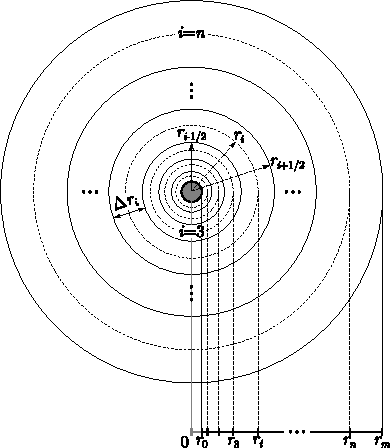
\includegraphics[height=5cm]{domain}
  \end{tabular}
  & \begin{tabular}{l}
    \parbox{0.5\linewidth}{%  change the parbox width as appropiate
    Some descriptions:}
  \end{tabular}  \\
\end{tabular}
\end{frame}

\subsection{Numerical implementation of CDE equation}
\begin{frame}
\end{frame}

\subsection{Other solute uptake models}
\begin{frame}
\end{frame}

\subsection{Scenarios}
\begin{frame}
\end{frame}

\subsection{Other analysis}
\begin{frame}
\frametitle{Other analysis}
Sensitivity analysis

Statistical difference
\end{frame}

\section{Results}

\subsection{Linear VS non-linear}
\begin{frame}
\end{frame}

\subsection{Models comparison}
\begin{frame}
\end{frame}

\subsection{Models results}
\begin{frame}
\end{frame}

\subsection{Sensitivity analysis}
\begin{frame}
\end{frame}

\section{Conclusions}
\subsection{Conclusions}
\begin{frame}
\end{frame}

\end{document}
